\documentclass[border=2mm]{standalone}
\usepackage{tikz}

\begin{document}

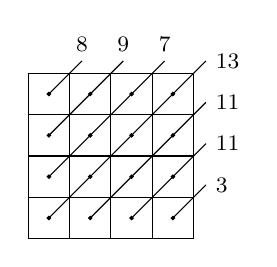
\begin{tikzpicture}[scale=0.7]
% Draw background grid
\draw[thin,color=black,step=.75cm] (0,0) grid (3,3);

% Place dots at centers of each grid cell (4x4 grid of points)
% Bottom row (y = 0.375)
\filldraw[fill=black] (0.375,0.375) circle (0.3mm);
\filldraw[fill=black] (1.125,0.375) circle (0.3mm);
\filldraw[fill=black] (1.875,0.375) circle (0.3mm);
\filldraw[fill=black] (2.625,0.375) circle (0.3mm);

% Second row (y = 1.125)
\filldraw[fill=black] (0.375,1.125) circle (0.3mm);
\filldraw[fill=black] (1.125,1.125) circle (0.3mm);
\filldraw[fill=black] (1.875,1.125) circle (0.3mm);
\filldraw[fill=black] (2.625,1.125) circle (0.3mm);

% Third row (y = 1.875)
\filldraw[fill=black] (0.375,1.875) circle (0.3mm);
\filldraw[fill=black] (1.125,1.875) circle (0.3mm);
\filldraw[fill=black] (1.875,1.875) circle (0.3mm);
\filldraw[fill=black] (2.625,1.875) circle (0.3mm);

% Top row (y = 2.625)
\filldraw[fill=black] (0.375,2.625) circle (0.3mm);
\filldraw[fill=black] (1.125,2.625) circle (0.3mm);
\filldraw[fill=black] (1.875,2.625) circle (0.3mm);
\filldraw[fill=black] (2.625,2.625) circle (0.3mm);

% Draw lines from left/bottom points to outside labels
\draw[thin, color=black] (0.375,0.375) -- (3.225,3.225) node[right] {{\footnotesize $13$}};
\draw[thin, color=black] (1.125,0.375) -- (3.225,2.475) node[right] {{\footnotesize $11$}};
\draw[thin, color=black] (1.875,0.375) -- (3.225,1.725) node[right] {{\footnotesize $11$}};
\draw[thin, color=black] (2.625,0.375) -- (3.225,0.975) node[right] {{\footnotesize $3$}};

\draw[thin, color=black] (0.375,1.125) -- (2.475,3.225) node[above] {{\footnotesize $7$}};
\draw[thin, color=black] (0.375,1.875) -- (1.725,3.225) node[above] {{\footnotesize $9$}};
\draw[thin, color=black] (0.375,2.625) -- (0.975,3.225) node[above] {{\footnotesize $8$}};
\end{tikzpicture}

\end{document}
